\chapter{Esitystyyli}%
\label{ch:esitystyyli}

Tekstin sisällön lisäksi esitystyyli vaikuttaa suuresti viestinnän onnistumiseen. Ulkoasu ja kirjoitustyyli antavat työstä ja kirjoittajasta kuvan, toivottavasti hyvän.

\section{Teksti}

Älä suotta murehdi tekstin asettelusta, tämä pohja hoitaa sen jo valmiiksi. Kirjoitustyylin perusohjeet ovat:

\begin{itemize}
\item Ajattele lukijaa aina tekstiä kirjoittaessasi ja johdattele häntä riittävästi. Anna ensin yleiskuva ja liitä siihen yksityiskohdat.
\item Korosta tärkeimmät asiat, esimerkiksi nostamalla ne omiksi luvuikseen (\verbcommand{section}, \verbcommand{subsection}), poimimalla taulukkoon tai selittämällä kuvan avulla. Tekstissä käytä korostamiseen kursivointia (\verbcommand{emph}), mutta älä korosta liikaa.
\item Vältä pitkiä virkkeitä ja monimutkaisia lauserakenteita. Piste on paras välimerkki.
\item Suosi aktiivimuodossa olevia verbejä ja sijoita ne lauseen alkupuolelle. Älä kuitenkaan käytä yksikön 1. persoonaa (minä) kuin alkusanoissa.
\item Vältä kapulakielisiä ilmauksia ja ammattislangia. Sano asiat suoraan. Käytä vakiintunutta teknistä sanastoa, merkintöjä ja neutraalia asiatyyliä.
\item Lukujen ja alalukujen tulee olla vähintään kahden kappaleen mittaisia ja mielellään keskenään tasapainoisia. Kappale muodostuu aina useammasta kuin yhdestä virkkeestä.
\item Luvut ja alaluvut numeroidaan korkeintaan kolmannelle tasolle (\verbcommand{subsection}) asti, esimerkiksi 4.4.2. Pohja huolehtii tästäkin automaattisesti.
\item Lyhenteitä ei tulisi käyttää liikaa. Käytä lyhenteissä pieniä ja isoja kirjaimia johdonmukaisesti.
\end{itemize}

\section{Lauseympäristöt}

Tiedostossa \code{tauthesis.cls} on määritelty lauseympäristöjä matemaattisen
tekstin kirjoittamista varten. Näistä esimerkkeinä toimivat suomen- ja
englanninkieliset lauseet~\ref{lause:pythagoras} ja \ref{theorem:pythagoras}.

\begin{lause}[Pythagoraan lause]\label{lause:pythagoras}
    Suorakulmaisen kolmion sivujen \(a\), \(b\) ja \(c\) pituuksille on voimassa yhtälö
    \begin{equation}\label{yht:pythagoras}
        a^2 + b^2 = c^2\,,
    \end{equation}
    jos \(c\) on hypotenuusa.
\end{lause}

\begin{theorem}[Pythagorean theorem]\label{theorem:pythagoras}
    For the sides of a right triangle, \(a\), \(b\) and \(c\), the equation
    \begin{equation}\label{eq:pythagoras}
        a^2 + b^2 = c^2
    \end{equation}
    holds, if \(c\) is the hypotenuse.
\end{theorem}

Tällä hetkellä määritellyt ympäristöt ovat \code{määritelmä} (kyllä,
ääkköset hyväksytään), \code{lause}, \code{apulause}, \code{seurauslause} ja
\code{esimerkki}, sekä vastaavat englanninkieliset ympäristöt \code{definition},
\code{theorem}, \code{lemma}, \code{corollary} ja \code{example}. Näitä on
suotavaa käyttää silloin, kun tekstissä esitellään jokin tärkeä tulos tai
määritelmä, johon tarvitsee viitata myöhemmin. Liika lauseympäristöjen käyttö
johtaa kuitenkin listamaiseen Landaun kirjoitustyyliin, joka ei ole kovin
helppolukuista, ja on sopivaa vain referenssityylisissä teksteissä, joista vain
haetaan faktoja. Diplomityö ei ole tällainen tekstityyppi.


\section{Kuvat}

Kaikkiin kuviin täytyy viitata tekstissä. Kuvan avulla voidaan esittää tietoa tiiviissä muodossa, mutta kuvan täytyy olla merkityksellinen työn sisällön kannalta ja kuva täytyy selittää tekstissä. Viittaus on mielellään samalla sivulla kuin kuva tai sitä ennen. Kuvat ja taulukot numeroidaan ja sijoitetaan pääsääntöisesti sivun yläreunaan, oman harkinnan mukaan. \LaTeX{}issa tämä tapahtuu sijoittamalla \verbcommand{caption}-komentoa seuraavalle riville \verbcommand{label}-komennon, jonka argumentti on kyseisen kuvan (tai taulukon) yksikäsitteinen tunniste. Viittaaminen tapahtuu \verbcommand{ref}-komennolla, johon syötetään haluttu tunniste. Lukua ei saa aloittaa (eikä mielellään lopettaa) kuvalla, taulukolla, kaavalla tai luettelolla, vaan sen ympärillä on oltava tekstiä. Kuvateksti sijoitetaan kuvan alle.

Kuvan keskeinen sisältö on selitettävä tekstissä, jotta sen sanomasta ei jää epäselvyyttä. Analysointiohjelmistojen tuottamat kuvat vaativat useimmiten muokkausta, kuten kuvassa \ref{fig:huolittelu}. Kuvan tekstien on oltava luettavissa, ja niiden kooksi suositellaan samaa kuin muussa tekstissä, 11 pt. Pyri siihen, että myös harmaasävyissä tulostettu kopio on luettava ja selkeä. Suosi vektorimuotoisia kuvatiedostotyyppejä \texttt{.eps} ja \texttt{.pdf} (\LaTeX{} ei syö \texttt{.svg}-tiedostoja\ldots), sillä niitä voi skaalata helposti laadun heikkenemättä. \LaTeX{} sisältää myös erittäin ilmaisuvoimaisia paketteja vektorigrafiikan (\texttt{tikz}) \parencite{tikz} ja kuvaajien (\texttt{pgfplots}) \parencite{pgfplots} piirtämiseen. Kuvassa \ref{fig:pgf-esimerkki} esitetään esimerkki jälkimmäisen avulla luodusta kuvaajasta.

\begin{figure}
\centering
%\begin{subfigure}{0.49\textwidth}
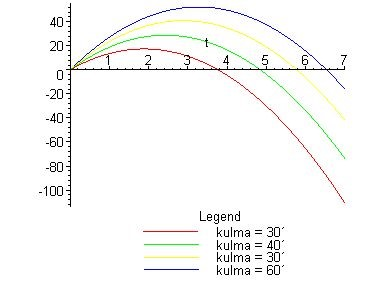
\includegraphics[alt={Esimerkki huonosti tehdystä muokkaamattomasta kuvasta.},width=0.9\linewidth]{images/bad-example.jpg}
%\end{subfigure}
%\begin{subfigure}{0.49\textwidth}
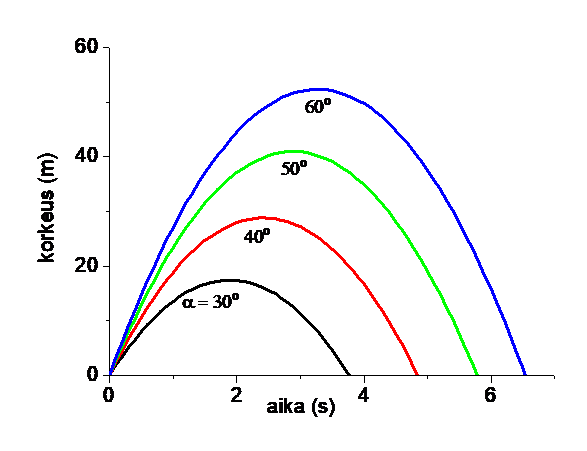
\includegraphics[alt={Esimerkki hyvin tehdystä, nykyistä esitystä varten muokatusta kuvasta.},width=0.9\linewidth]{images/good-example.png}
%\end{subfigure}
\caption[Tämä on lyhyt kuvateksti.]{Kuvaaja on hyvä muokata julkaisukelpoiseksi. Vasemmalla on esitetty muokkaamaton kuvaaja ja oikealla muokattu.}
\label{fig:huolittelu}
\end{figure}

\section{Taulukot}

Taulukot sopivat hyvin erityisesti numeerisen informaation esittämiseen tiiviissä muodossa. Kuvien tapaan taulukot numeroidaan ja varustetaan otsikolla, kuten taulukossa. Taulukkoteksti sijoitetaan samalle sivulle taulukon kanssa ja taulukon yläpuolelle. Suureet, lyhenteet ja symbolit selitetään tarvittaessa tekstissä. Kaikkiin taulukoihin on viitattava tekstissä, mieluummin ennen taulukkoa. Taulukon keskeinen sanoma ja tulkintaohjeet selitetään tekstissä.

Taulukon sarakkeet otsikoidaan, ja suureet sekä yksiköt laitetaan näkyviin. Jos otsikkoriviä tarvitsee erottaa muusta taulukosta, tee se korostamalla (\verbcommand{emph}). Taulukon järjestyksellä on suuri merkitys. Jokaista solua ei pidä ympäröidä reunaviivalla, koska taulukosta tulee raskaslukuinen. Lisää vaakaviiva taulukon ylä- ja alareunaan. Vaakaviivoja voi käyttää esimerkiksi 4--5 rivin välein, ellei tietoja muuten ole jaettu kategorioihin tai selkeys sitä vaadi. Sarakkeen numeroarvot tasataan desimaalipilkun kohdalta, jolloin arvoja on helppo vertailla. Tämä tapahtuu \LaTeX{}issa helposti \texttt{siunitx}-paketin \parencite{siunitx} taulukkomateriaalin avulla. Tavoitteena on, että suureet ilmaistaan SI-yksikössä ja käytetään joko vakiintuneita etuliitteitä tai kymmenen potenssin muotoja siten, että ne voidaan laittaa otsikkoriville (katso tässäkin \texttt{siunitx}). Muutamia suosituksia taulukoiden ja kuvien käytöstä löydät lähteestä \parencite{pubadvice2009}.

\begin{table}
\centering
\caption{Esimerkki höyrystysolosuhteista kahdessa ohutkalvorakenteessa.}
\label{tab:taulukkoesimerkki}
% Making scarce use of table lines is recommended
% for clarity. Even the outer lines are generally
% not needed! Use the siunitx package provided
% S column type for easy decimal alignment.
%\begin{tabular}{c|S[table-format=3.1] S[table-format=1.2] S[table-format=2.1e-1] S[table-format=2.1] S[table-format=2.0]@{--}S[table-format=3.0] S[table-format=1.1]}
%    \hline
%    aine & {paksuus} & {korjauskerroin} & {paine} & {lämpötila} & \multicolumn{2}{c}{virta} & {nopeus} \\[-0.5ex]
    % The syntax \\[<length>] inserts a vertical
    % space of <length> in addition to the normal
    % new line action provided by \\. This should
    % apply in any situation.
%    & {(\si{\nano\metre})} & & {(\si{\milli\bar})} & {(\si{\degreeCelsius})} & \multicolumn{2}{c}{(\si{\milli\ampere})} & {(\si{\nano\metre\per\second})} \\\hline
%    SiO2 & 181.0 & 1.10 & 3.0e-5 & 90.6 & 20 & 23 & 0.2 \\
%    TiO2 & 122.1 & 1.55 & 15.0e-5 & 91.1 & 93 & 100 & 0.1 \\\hline
%\end{tabular}
\end{table}

\section{Matemaattiset merkinnät ja yhtälöt}

Käytä selvyyssyistä mieluummin numeroita kuin kirjaimia lukuarvoissa: esimerkiksi ''6 työvaihetta'' on selkeämpi ja parempi kuin ''kuusi työvaihetta''. Tuhaterottimen käyttö selkeyttää tekstiä, eli kirjoita 55~700~125 muodon 55700125 sijaan. Desimaalipilkkua edeltävä nolla tulee aina merkitä. Suomen kielessä käytetään virallisesti desimaalipilkkua, englannin kielessä desimaalipistettä. Näistäkin tämä pohja ja \texttt{siunitx} \parencite{siunitx} huolehtivat siististi, jos vain annat niiden (muista ottaa \texttt{siunitx} käyttöön).

Numeroiden tavoin myös mittayksiköt kannattaa kirjoittaa lyhenteinä. Mittayksikön ja numeroarvon välissä on itse asiassa välilyöntiä lyhyempi väli, ja niiden tulee olla samalla rivillä. Taulukko tai kaavio on parempi esitystapa, jos tekstin sekaan tulee runsaasti numeroarvoja. Usein numeroarvoihin voi liittää laadullisen määreen, ja vastaavasti kaikkiin laadullisiin määreisiin (suuri, pieni, kallis, nopea) tulisi liittää numeroarvo kuvaamaan suuruusluokkaa. Numeroiden kanssa ei tarvitse käyttää sijapäätettä, jos seuraava sana on samassa sijassa (taivutusmuodossa), esimerkiksi ''jakautuu 10 osaan'' ja ''20 ja 50 sentin kolikot''. On myös tapauksia, joissa sijapääte pitää merkitä, esimerkiksi lauseessa ''osallistujia oli 7:stä eri maasta''.

Tekstissä tulee ensisijaisesti käyttää yleisesti tunnettuja ja hyvin määriteltyjä käsitteitä, joiden kirjoittamiseen on yleensä jokin vakiintunut merkintätapa tai symboli. Uudet käsitteet ja merkinnät pitää määritellä, kun ne esiintyvät tekstissä ensimmäisen kerran. Symboleissa ja mittayksiköissä isot ja pienet kirjaimet tarkoittavat eri asioita. Samaa symbolia ei tule käyttää monessa eri merkityksessä. Mittayksiköt merkitään selvästi.

Matemaattiset merkit ja kreikkalaiset kirjaimet löytyvät \LaTeX{}in makroista ja kaavamoodeista, kuten \(\Theta(n^2)\). Yksinkertaiset kaavat voivat olla osa virkettä (siis tekstiä) ja ilman numeroa. Esimerkkinä tekstistä erotetusta kaavasta Newtonin 2. peruslaki voidaan ilmaista muodossa
\begin{equation}\label{eq:newton2}
    m\mathbf{a} = \mathbf{F} \,,
\end{equation}
missä \(m\) on kappaleen massa, \(\mathbf{a}\) sen kiihtyvyys ja \(\mathbf{F}\) siihen kohdistuva nettovoima. Huomaa, että symbolien merkitys selitetään aina heti kaavan yhteydessä sillä tavalla kuin on luontevinta. Kaavat esitetään tarkoituksella eri fontilla ja matemaattiset symbolit pääosin kursivoidaan. Vektorit voidaan esittää lihavoituna, kuten edellä (tavallisinta painetussa tekstissä) tai nuolella varustettuna, kuten \(\vec{v}\). Dimensiollisia lukuja voidaan esittää \verbcommand{SI}-komennon avulla:
\begin{equation*}
    \norm{\mathbf{F}}
    =
    m\norm{\mathbf{a}}
    =
    \SI{10}{\kilogram} \cdot \SI{9.81}{\metre\per\second\squared}
    =
    \SI{98.1}{\newton} \,.
\end{equation*}

Matemaattinen kaava numeroidaan, jos se on omalla rivillään ja siihen viitataan muualla tekstissä, katso esimerkiksi kaava \eqref{eq:newton2}. Usein numero on tavallisten sulkujen sisällä ja tasattu oikeaan laitaan, kuten tässä ohjeessa. Matematiikan kirjoitusohjeiden ja englatilaisen kulttuuripiirin tavan mukaisesti kaavoihin sisällytetään välimerkit, kuten yhtälössä \eqref{eq:newton2} lopun pilkku. Toisinaan matemaattisen rakenteen edessä on tunniste, kuten Määritelmä 1 tai Lause 1 \parencite{matohje2009}. Nämä luodaan omilla \texttt{amsthm}-pakettiin pohjautuvilla ympäristöillään. Kaavojen ja muiden rakenteiden numerointi voi olla juokseva läpi koko tekstin ((1), (2), \ldots) tai aina yhden luvun sisällä ((1.1), (1.2), \ldots, (2.1), \ldots).

Älä aloita uutta virkettä matemaattisella symbolilla. Yleensä teknis-fysikaalisessa tekstissä kursivoidaan muuttujat, kuten \(x\) ja \(y\). Kursivoinneissa kannattaa luottaa \LaTeX{}in automatiikkaan \parencite{notsoshort}. Sen sijaan alkeisfunktioita, erikoisfunktioita ja operaattoreita merkitään tavallisella kirjasimella: \(\sin(2x + y)\) tai
\begin{equation*}
    \lim_{x \rightarrow -1}\frac{x^2 - 1}{x + 1} = -2 \,.
\end{equation*}
Kappaletta, tai varsinkaan lukua ei ole hyvä myöskään lopettaa kaavaan, kuvaan tai taulukkoon.

%Kemian symboleita tarvitseviakaan \LaTeX{} ei jätä pulaan. Molekyylikaavoja ja reaktioyhtälöitä, kuten \ce{CH3CH2CH2COOH} ja
%\begin{center}
%    \ce{N2 (g) + 3 H2 (g) <=> 2 NH3 (g)}
%\end{center}
%varten tarvitaan \texttt{mhchem}-paketti \parencite{mhchem}, ja kokonaisia rakennekaavoja varten \texttt{chemfig} \parencite{chemfig}. Esimerkkinä jälkimmäisestä voidaan esittää telluriumtetrafluoridin (\ce{TeF4}) Lewisin rakenne.
%\begin{center}
%    \chemfig{\lewis{0:,Te}
%    (-[:90]\lewis{0:2:4:,F})
%    (-[:270]\lewis{0:4:6:,F})
%    (<:[:135]\lewis{1:3:5:,F})
%    (<[:225]\lewis{3:5:7:,F})
%    }
%\end{center}
%Varsinkin rakennekaavojen latominen vaatii totuttelemista, mutta keinot ovat olemassa.

\section{Ohjelmat ja algoritmit}

Koodin kirjasinlajina käytetään \texttt{tasalevyistä kirjasinlajia}, jonka merkit ovat yhtä leveitä. Kun ohjelmakoodin tai algoritmin pituus on alle 10 riviä eikä siihen enää myöhemmin tekstissä viitata, se voidaan esittää kuten kaavat. Pidemmät, alle sivun mittaiset ohjelmakoodit tai algoritmit kirjoitetaan kuten Ohjelma \ref{prog:esimerkki}, otsikkona ''Ohjelma'' tai ''Algoritmi''.

Koodiin on hyvä lisätä muutamia kommentteja ja sisentää se johdonmukaisesti. Koodin toiminta selitetään aina myös juoksevassa tekstissä pääpiirteissään, lähinnä siitä esitetään muutamia avainhuomioita. Esimerkiksi \LaTeX{}in paketti \texttt{listings} \parencite{listings,notsoshort} osaa kätevästi sisällyttää sekä oikeita kooditiedostoja että pseudokoodia tekstiin, lisätä automaattisesti rivinumeroinnin ja korostaa monet varatut sanat. Käytä sitä kaiken koodin esittämiseen \LaTeX{}in avulla.

\renewcommand{\lstlistingname}{Ohjelma}
\lstinputlisting
    [
        float,
        caption={Esimerkki ohjelmakoodin esittämisestä.},
        label=prog:esimerkki,
        language=C,
        numbers=left,
        morekeywords={Kirjainpari},
        inputencoding=utf8,
    ]
    {code/esimerkkikoodi.c}

\section{Saavutettava opinnäytetyö}

Suomen laki vaatii Euroopan unionin saavutettavuusdirektiivin 2016/2102 mukaisesti, että sähköiseistä julkaisuista tehdään saavutettavia (järkevällä työmäärällä). Tämä pätee myös opinnäytetyöhösi, minkä vuoksi on hyvä tietää tai ottaa selvää työsi saavutettavuusvaatimuksista. Opinnäytetyön pohjan kirjoittaja tai ylläpitäjä ei ota minkäänlaista vastuuta puolestasi!

Tämä pohja pyrkii auttamaan lopullisen dokumentin saavutettavuuden parantamisessa niin paljon kuin mahdollista. Valitettavasti vuonna 2021 (ja luultavasti vuoteen 2024 asti) \LaTeX{} ei pysty tuottamaan PDF/UA standardin, tai edes hiukan vähemmän vaativien yliopiston ohjeiden mukaista tiedostoa. Pääsyynä on, että \LaTeX{} heittää muistin säästämiseksi paljon tähän tarvittavasta dokumentin rakenneinformaatiosta romukoppaan heti, kun mahdollista (muistiongelma oli todellinen 80- ja 90-luvuilla). Kaikkea toivoa ei kuitenkaan ole menetetty, ja työssä pitäisi silti pyrkiä maksimoimaan saavutettavuus!

Kuten opinnäytetyön ulkoasun kanssa, tämä pohja pyrkii automatisoimaan monet saavutettavuusratkaisut puolestasi. Muutamat seikat, joihin pitää kiinnittää huomiota kirjoittaessa ovat
\begin{enumerate}
\item selkeän ja merkitykseltään yksikäsitteisen kielen käyttäminen, sekä keskeisen informaation välittäminen sanoin, eikä vain visuaalisin keinoin,
\item vaihtoehtoisten tekstien (tekstivastineiden, alt-tekstien) kirjoittaminen \emph{kaikille} työssä käyttämillesi kuville,
\item dokumentin metadatakentistä otsikon ja pääkielen ylläpitäminen,
\item matematiikan automaattisen tekstivastineratkaisun kannalta yhteensopivien matematiikkaympäristöjen käyttäminen.
\end{enumerate}
Noudata näissä kohdissa seuraavia ohjeita.
\begin{enumerate}
\item Tee kuten yllä kuvattiin. Käytä tarvittaessa ulkoisia palveluja tekstisi helppolukuisuuden arvioimisen tukena.
\item Huomaa, että kuvaotsikko ja tekstivastine kirjoitetaan palvelemaan eri tarkoituksia ja että tekstivastine ei koskaan saa olla vain kuvaotsikon kopio! (Ruudunlukijat sitä paitsi lukevat kuvaotsikot tekstivastineen lisäksi.) Kuvaile tekstivastineessa kuvan visuaalista sisältöä runsaasti, mutta keskity myös vain olennaisimpiin merkityksiin, joita kuva välittää.
\item Pidä dokumentin metadatakentät aivan \texttt{main.tex}-tiedoston alussa aina ajan tasalla.
\item Älä käytä vanhoja \TeX{}-tyylisiä \verb+$...$+- ja \verb+$$...$$+-ympäristöjä matematiikkaa varten. Käytä niiden sijaan \LaTeX{}-tyylisiä \verb+\(...\)+- ja \verb+\[...\]+-ympäristöjä. Keskitetyn matematiikan tupladollareita ei muutenkaan pitäisi käyttää.

Suurin osa \texttt{amsmath}-paketin matematiikkaympäristöistä, kuten \texttt{equation}, \texttt{equation*} ja \texttt{align} saavat tekstivastineet automaattisesti oikein. Vastaavasti muissa paketeissa määriteltyjä matematiikkaympäristöjä ei tueta! Matematiikan tekstivastine kaikissa matematiikkaympäristöissä on yksinkertaisesti sen \LaTeX{}-lähdekoodi, kunnes parempi ratkaisu saadaan aikaiseksi.
\end{enumerate}
